\section{Algoritmo exacto}
\subsection{Desarrollo}
Para el desarrollo del algoritmo exacto, nos percatamos de la similitud del problema con el ejercicio número 3 del TP1 (optimizar el número de camiones para transportar quimicos sin que se exeda un nivel de peligrosidad m).

Podríamos modelar al problema como un grafo.
Supongamos a los productos como nodos del grafo, y al peso de las aristas como la peligrosidad de los 2 productos (nodos) incidentes a ella (si no hay arista entre 2 nodos, significa que no aporta peso intraparticion, es decir, en la analogía, esos 2 nodos tendrían pelogrisidad 0 entre sí).\\
De esta forma, si pensamos en que tenemos que tomar conjutnos disjuntos de nodos, esto sería similar a la selección de productos en distintos camiones. La única diferencia que se presenta, es que no hay un umbral de peligrosidad, y, como tenemos que dividir a los nodos en k conjutnos, el equivalente a la analogía sería que el número de camiones sea constante y lo que hace a una solución mejor que otra, es una menor peligrosidad total (con peligrosidad total nos referimos a la suma de las peligrosidades de cada camion).

Aplicamos algunas podas para mejorar los tiempos de ejecución:
\begin{enumerate}
\item Poda de optimalidad. Esta poda evita revisar configuraciones de conjuntos de partición, si se detecto que el peso total de la partición que se está revisando ya excedió otro anteriormente calculado.
\item Poda de invalidez. Esta poda evita que se revisen particiones de mas de k conjuntos, ya que son inválidas por definición.
\item Cota greedy previa: Con esta cota, ingresamos de manera golosa nodos entre k conjuntos, para que nos devuelva una configuración posible de respuesta. Si bien la probabilidad de que esta sea la solución optima es muy baja, la probabilidad de que esa cota devuelva la peor configuración también lo es. Si la cota devolviese la peor solución habría sido como si no hubiera existido, porque no hubiera acotado más al problema.
\end{enumerate}

\subsection{Complejidad}

Algunas aclaraciones previas al análisis de complejidad del ejercicio:

\begin{enumerate}

\item Nodo es int, Nodos es Vector(int), Conjunto es Vector(int), Particion es Vector(Conjunto), Pesos es Vector(Vector(int))
\item Asumo que las operaciones de vector PonerAlFinal(push\_back), sacarUltimo (pop\_back), Constructor por defecto (sin indicador de tamaño), el operator[], size y la asignación (por referencia) tienen complejidad $O(1)$. Cabe aclarar que esto no es siempre cierto para push\_back, pero como se hicieron los pertinentes pedidos de reserva de memoria, para simplificar el argumento voy a tomarlo como tal.
\item La subrutina pesoDeParticion(Particion,Pesos) comprueba el peso total de una partición, es decir, la suma de los pesos de las aristas intraparticion, Particion y Pesos se pasan por referencia. La función que caracteriza su complejidad pertenece a O($n^2$), donde $n$ son los nodos dispersos por los conjutnos. La función responde a este pseudo codigo:
\bigskip
\begin{lstlisting}
int pesoDeParticion(Particion,Pesos)
	acum <- 0
	Para cada conjunto de la particion
		acum <- acum + pesoDeConjutno(conjunto,pesos)
Retornar acum

int pesoDeConjunto(conjunto, pesos)
	Si conjunto.length < 2
		Retornar 0

	acum <- 0
	Para i (nodo) desde 0 hasta length del conjunto
		Para j (nodo) desde i+1 hasta length del conjunto
			acum <- acum + pesoDeArista(conjunto[i],conjunto[j],pesos)
Retornar acum
\end{lstlisting}
\end{enumerate}

Donde pesoDeArista, consulta la posicion del vector pesos indicada por los nodos, en $O(1)$.

Dicho esto, el análisis de la complejidad del algoritmo de backtracking esta sujeta a esta función recursiva:

\[ T(i) = \left\{ \begin{array}{ll}
         (n-(i+1)+1)T(i-1) + O((n-i)^2) & \mbox{, si $0 < i < n$}\\
         O(n^2) & \mbox{, si $i = 0$}\end{array} \right. \]
Cancelando los índices:

\[ T(i) = \left\{ \begin{array}{ll}
         (n-i)T(i-1) + O((n-i)^2) & \mbox{, si $0 < i < n$}\\
         O(n^2) & \mbox{, si $i = 0$}\end{array} \right. \]

Donde i es el número del próximo nodo a ser puesto en los distintos conjuntos de la partición. Si el for principal del algoritmo esta sujeto a la cantidad de conjuntos, la pregunta es, ¿Por qué la función de recursión no lo está también? La respuesta yace en el análisis del peor caso. La máxima cantidad de llamados recursivos ocurre cuando cada conjunto tiene 1 solo nodo, dado que se genera la mayor cantidad de conjuntos para dicho llamado recursivo. Si el próximo nodo a ser analizado es el i, entonces los elementos i+1...n ya fueron colocados en distintos conjutnos, por ende la cantidad en peor situación es (n-(i+1)). Sumado a esto, ocurre un último llamado recursivo en el que se coloca el nodo i en un nuevo conjunto, por ello el +1 multiplicando a T(i-1). El segundo término de T(i) describe la complejidad de hacer pesoDePartición en dicho paso. El caso base es hacer pesoDePartición con todos los nodos colocados.\newline
\indent Supongamos una cantidad n (con n $\geq$ 5 para el caso particular de esta demostración) de nodos, esto implica que el último nodo es $p_n-1$, o el nodo (n-1), desarrollando la función desde (n-1) se obtiene lo siguiente:

$T(n-1) = (n-(n-1))T(n-2) + O((n-(n-1))^2) = 1T(n-1) + O(1) = 2T(n-3) + O(2^2) + O(1) = $

$2(3T(n-4) + O(3^2)) + O(2^2) + O(1) = 3!T(n-4) + O(2*3^2) + O(1) = $

$3!(4T(n-5) + O(4^2)) + O(2*3^2) + O(1) = 4!T(n-5) + O(3!*4^2) + O(2!*3^2) + O(0!*1^2) =$

$...(i = 0)... = (n-1)!T(0) + \sum\limits_{k=1}^{n-1} O((k-1)!*k^2) = (n-1)!T(0) + O(\sum\limits_{k=1}^{n-1} (k!*k))$

Por lo demostrado en el ejercicio 1.f de la Práctica 1, por propiedades de la función O y de la función factorial, nos queda que:

$(n-1)!T(0) + O(((n-1)+1)!) - 1 = (n-1)!O(n^2) + O(n!) - 1 = O((n-1)*n^2)) + O(n! - 1) =$

$O(n*n!) + O(n!)$

Además, como n $\in \aleph \implies ( n*n! \geq n! \iff n \geq 1)$ lo cual es cierto ya que n es un natural.
Por ende, $O(n*n!) + O(n!) = O(max\{n*n!,n!\}) = O(n*n!) = T(n-1)$ que es de donde arrancamos. Y $T(n-1)$ define la complejidad del algoritmo. Finalmente, el algoritmo tiene complejidad O($n*n!$).

Esto no es todo ya que a esta complejidad hay que sumarle el costo temporal del algoritmo \textbf{generarParticionInicial}. Dicho algoritmo itera los n nodos, y los va guardando en uno de los k conjuntos de la particion. Una vez realizado eso calcula el peso de la partición y lo devuelve.
Por ende, esta primer cota aplicada tiene costo lineal en la cantidad de nodos por iterarlos + costo cuadratico de calculo de peso de particion (complejidad al principio de esta sección). Para una mayor facilidad el pseudocódigo es el siguiente:

\begin{lstlisting}
//Recibe un conjunto de conjutnos vacia, nodos, pesos, y el valor k

int generarParticionInicial(particion, nodos, pesos, k)
	incrementarParticion <- true
	i <- 0

	Para cada nodo hacer:
			Si incrementarParticion
				agregar un conjunto al final de particion

			agregar nodo al conjunto i de la particion

			i++;
			Si i == k
				i <- 0;
				incrementarParticion<-false;

return pesoDeParticion(particion, pesos);
\end{lstlisting}

En conclusión, si decimos que $f(n)$ es la función que caracteriza la complejidad del algoritmo que resuelve el problema, podemos decir que $f(n) = O(n*n!) + O(n^2)$. Sabemos, por el ejercicio 3.b de la Práctica 2, que dado r $\in \aleph$, $n^r \in O(n!) \implies n^r \in O(n*n!)$. Entonces, $f(n) = O(n*n!)$.

Si bien la cota de lo que podría tomar resolver el problema es holgada, recordemos que realmente se llega a ella en el caso en que ningún nodo pueda estar en el mismo conjunto que otro, ya que se deben descartar todas las particiones posibles antes de poder decir con seguridad que es la manera más eficiente de acomodar los nodos.

\subsection{Experimentación}
Para la experimentacion, se realizaron distintos escenarios de test. Cada escenario contiene valores que son producto de distintas tomas de datos del algoritmo en ejecución.
Se hicieron pruebas del algoritmo, con las podas aplicadas y sin ellas, permitiendo observarse la gran diferencia que estas hacen.

Como es sabido, la computadora en la que se realizaron las mediciones, no está atentiendo nuestro proceso únicamente. Es por eso, que realizar una única medición de cada instancia no nos asegura fidelidad.\\
\indent Para aminorizar esta falencia, se repitió cada instancia de cada caso de test de cada escenario, un total de 100 veces, y se tomó el mejor tiempo.\\
Notar que tomar el mejor tiempo (en lugar del promedio) no es una mala desición, ya que entre 2 mediciones de tiempos distintas, t1 y t2, si t1 es menor a t2, eso nos asegura que en t1 el procesador estuvo más focalizado en nuestro proceso, y por ende, es una medición más fiel del mismo.

Para realizar las mediciónes, se realizó un generador de instancias aleatorias, que dada una cantidad de nodos (n), una cantidad de aristas (m) y un entero (k), genera de forma aleatoria m aristas, tomando para cada una, 2 nodos de n, que no tengan ya una arista entre ellos.

Debido a que el algoritmo coloca un peso de 0 (cero) entre nodos que no sean adyacentes (explicado en la primer sección), esto hace que el tiempo de ejecución \textit{\textbf{de peor caso}} no dependa de la cantida de aristas, ya que siempre, para cualquier grafo de entrada, el grafo a computar termina siendo un grafo completo y por ende la cantidad de aristas es:

\begin{center}
\LARGE $\frac{(n * (n-1))}{2}$ \\
\end{center}


\underline{Sin más, detallamos los casos de test:}\\

Los siguientes escenarios son mediciones hechas del algoritmo, con las podas/cotas aplicadas.

\indent ESCENARIO PARA K = 5
	\begin{figure}[h]
		\begin{center}
		   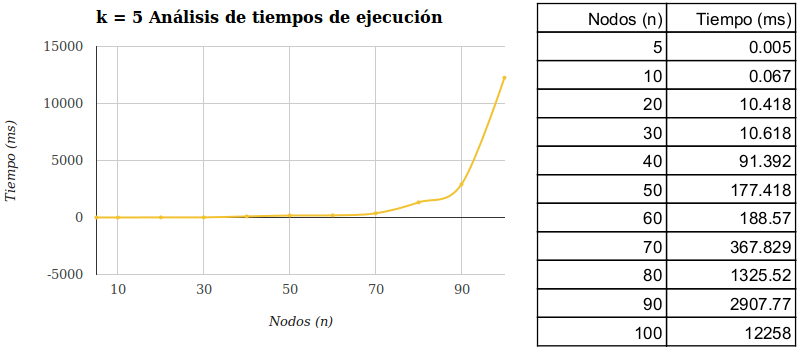
\includegraphics[scale=0.70]{ejercicio2/k5.png}
		\end{center}
	\end{figure}

Debido a que la cota inicial va ingresando de a un elemento en cada uno de los k conjuntos, a \textbf{mayor} k, menor será el peso total de la partición, ya que los nodos estarán mas divididos, y por ende, habrá menos aristas intrapartición. (Claro está que en el peor de los casos, los nodos que no están en el mismo conjunto son aquellos que no tienen peso (estrictamente hablando, tienen peso = 0), pero hay una alta probabilidad de que esto no pasé, por eso, es una cota).

\newpage ESCENARIO CON K = 25
	\begin{figure}[h]
		\begin{center}
		   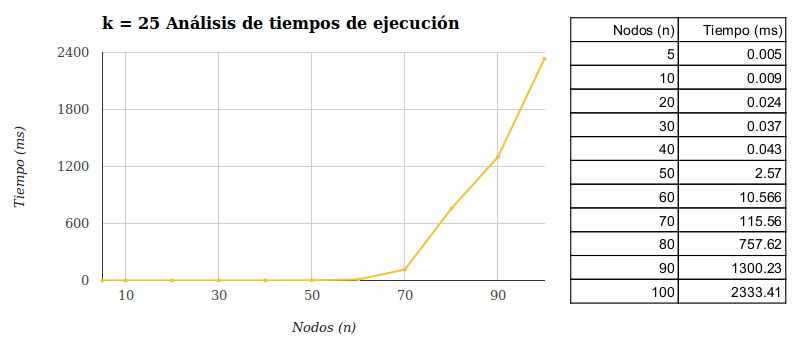
\includegraphics[scale=0.80]{ejercicio2/k25.png}
		\end{center}
	\end{figure}

Comparando los tiempos con el gráfico anterior, y tal como se dijo, las cotas hacen mayor efecto para un k más grande. En este caso, un k 5 veces más grande.\\
\\

\indent ESCENARIO CON K = 75
	\begin{figure}[h]
		\begin{center}
		   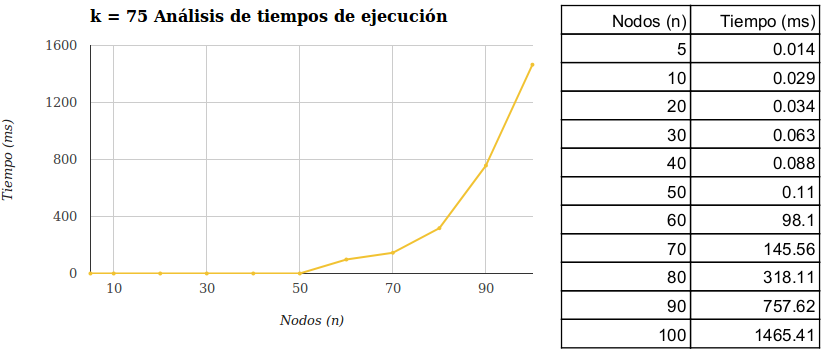
\includegraphics[scale=0.80]{ejercicio2/k75.png}
		\end{center}
	\end{figure}

En este gráfico podemos ver que, por ejemplo, en instancias de 60 nodos nos encontramos con un caso en el que las podas/cotas no funcionaron mejor que antes, como si lo hizo en el gráfico anterior (k = 25) para una instancia de igual tamaño ya que los tiempos no fueron mejores, pero, debido a que los casos en los que las podas/cotas no nos ayudan demasiado son menos probables que los que sí (y por eso se eligieron esas podas/cotas), más adelante, los tiempos muestran que sí volvieron a hacer efecto, observando que por ejemplo, para instancias de 90 nodos, el tiempo se redujo aproximandamente un 50\%, principalmente la cota inicial, que depende vitálmente de k.

\newpage \indent ESCENARIO CON K = 200
	\begin{figure}[h]
		\begin{center}
		   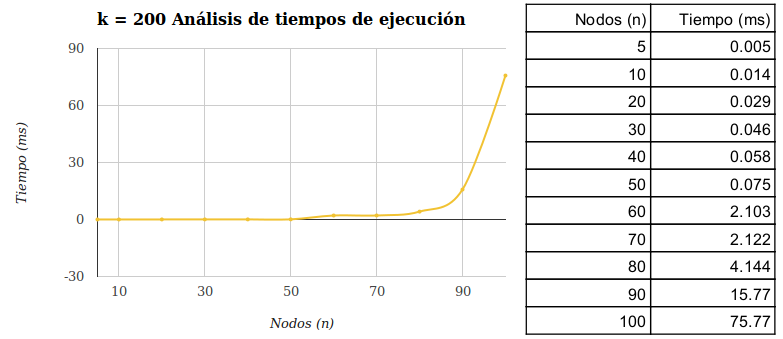
\includegraphics[scale=0.80]{ejercicio2/k200.png}
		\end{center}
	\end{figure}


Finalmente, en el siguiente gráfico se puede comparar y apreciar la relación entre los 4 gráficos detallados, donde se puede apreciar, que a un mayor k, la cota responde bien:

	\begin{figure}[h]
		\begin{center}
		   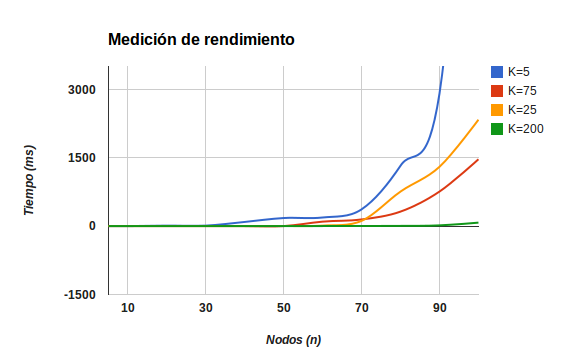
\includegraphics[scale=0.80]{ejercicio2/todasK.png}
		\end{center}
	\end{figure}

Cada una de las instancias probadas se realizó con distintas cantidades de aristas. Más especificamente entre 20 y 80 aristas, a excepción de los casos de muy pocos nodos (5 o 10) en los que no es posible aplicar tantas ya que se \textbf{llena} el grafo antes.Esta variación no produjo relevantes cambios en los tiempos.\\ \\

\underline{Algoritmo exacto \textit{\textbf{sin podas y cotas}}}\\
En cuanto al algoritmo exacto, sacandole TODAS las podas y cotas, comenzamos a hacer mediciones, pero con instancias chicas (en cuanto a cantidad de nodos), el tiempo de computo se disparaba fuertemente, tal como la complejidad lo sugiere, y demandaba días terminar todos los experimentos, pero, definitivamente, el salto de tiempo entre instancias cada vez mas grandes era realmente exponencial, y el tiempo total de computo era muy distinto al computado con las podas aplicadas, a pesar de que eran exactamente las mismas instancias. Eso podía notarse al poco tiempo en el que la misma instancia, con podas, ya había terminado.
